\documentclass[14pt]{extbook}
\usepackage{multicol, enumerate, enumitem, hyperref, color, soul, setspace, parskip, fancyhdr} %General Packages
\usepackage{amssymb, amsthm, amsmath, latexsym, units, mathtools} %Math Packages
\everymath{\displaystyle} %All math in Display Style
% Packages with additional options
\usepackage[headsep=0.5cm,headheight=12pt, left=1 in,right= 1 in,top= 1 in,bottom= 1 in]{geometry}
\usepackage[usenames,dvipsnames]{xcolor}
\usepackage{dashrule}  % Package to use the command below to create lines between items
\newcommand{\litem}[1]{\item#1\hspace*{-1cm}\rule{\textwidth}{0.4pt}}
\pagestyle{fancy}
\lhead{Module5}
\chead{}
\rhead{Version A}
\lfoot{3697-2165}
\cfoot{}
\rfoot{test}
\begin{document}

\begin{enumerate}
\litem{
Solve the radical equation below. Then, choose the interval(s) that the solution(s) belongs to.\[ \sqrt{-72 x^2 - 20} - \sqrt{77 x} = 0 \]\begin{enumerate}[label=\Alph*.]
\item \( x_1 \in [0.43, 0.89] \text{ and } x_2 \in [0.22,0.79] \)
\item \( x_1 \in [-0.88, -0.54] \text{ and } x_2 \in [-0.69,-0.21] \)
\item \( \text{All solutions lead to invalid or complex values in the equation.} \)
\item \( x \in [-0.88,-0.54] \)
\item \( x \in [-0.47,-0.41] \)

\end{enumerate} }
\litem{
What is the domain of the function below?\[ f(x) = \sqrt[7]{-7 x - 6} \]\begin{enumerate}[label=\Alph*.]
\item \( \text{The domain is } (-\infty, a], \text{   where } a \in [-0.9, -0.77] \)
\item \( \text{The domain is } [a, \infty), \text{   where } a \in [-1.13, -0.8] \)
\item \( (-\infty, \infty) \)
\item \( \text{The domain is } (-\infty, a], \text{   where } a \in [-1.37, -1.1] \)
\item \( \text{The domain is } [a, \infty), \text{   where } a \in [-1.81, -0.93] \)

\end{enumerate} }
\litem{
Choose the equation of the function graphed below.
\begin{center}
    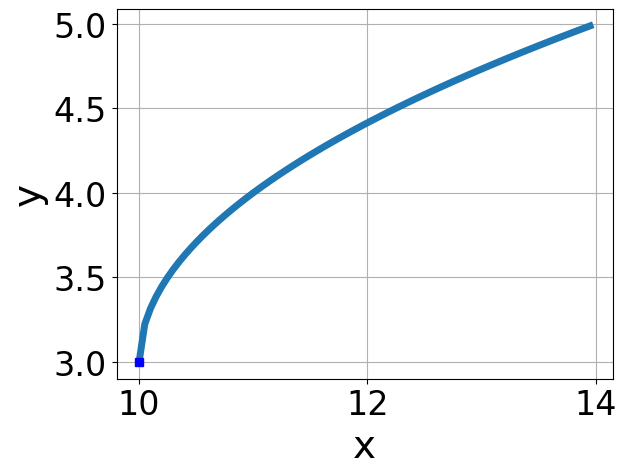
\includegraphics[width=0.5\textwidth]{../Figures/radicalGraphToEquationA.png}
\end{center}
\begin{enumerate}[label=\Alph*.]
\item \( f(x) = \sqrt[3]{x + 14} - 3 \)
\item \( f(x) = - \sqrt[3]{x - 14} - 3 \)
\item \( f(x) = - \sqrt[3]{x + 14} - 3 \)
\item \( f(x) = \sqrt[3]{x - 14} - 3 \)
\item \( \text{None of the above} \)

\end{enumerate} }
\litem{
Solve the radical equation below. Then, choose the interval(s) that the solution(s) belongs to.\[ \sqrt{-12 x^2 - 10} - \sqrt{34 x} = 0 \]\begin{enumerate}[label=\Alph*.]
\item \( x_1 \in [2.5, 3.5] \text{ and } x_2 \in [0,2.2] \)
\item \( x \in [-1.33,1.67] \)
\item \( x_1 \in [-5.5, -0.5] \text{ and } x_2 \in [-1.7,-0.2] \)
\item \( x \in [-5.5,-0.5] \)
\item \( \text{All solutions lead to invalid or complex values in the equation.} \)

\end{enumerate} }
\litem{
Choose the equation of the function graphed below.
\begin{center}
    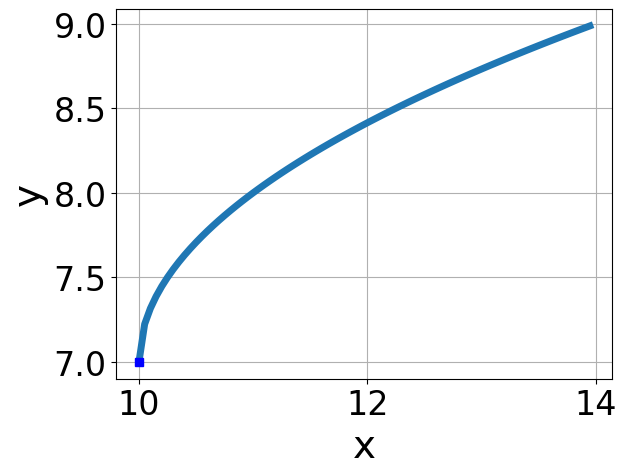
\includegraphics[width=0.5\textwidth]{../Figures/radicalGraphToEquationCopyA.png}
\end{center}
\begin{enumerate}[label=\Alph*.]
\item \( f(x) = - \sqrt{x - 10} + 7 \)
\item \( f(x) = \sqrt{x - 10} + 7 \)
\item \( f(x) = - \sqrt{x + 10} + 7 \)
\item \( f(x) = \sqrt{x + 10} + 7 \)
\item \( \text{None of the above} \)

\end{enumerate} }
\litem{
What is the domain of the function below?\[ f(x) = \sqrt[5]{-5 x + 7} \]\begin{enumerate}[label=\Alph*.]
\item \( \text{The domain is } (-\infty, a], \text{   where } a \in [-1.1, 1.1] \)
\item \( \text{The domain is } [a, \infty), \text{   where } a \in [-0.23, 1.25] \)
\item \( \text{The domain is } [a, \infty), \text{   where } a \in [1.07, 2.59] \)
\item \( \text{The domain is } (-\infty, a], \text{   where } a \in [0.8, 3.6] \)
\item \( (-\infty, \infty) \)

\end{enumerate} }
\litem{
Choose the graph of the equation below.\[ f(x) = - \sqrt[3]{x + 14} - 5 \]\begin{enumerate}[label=\Alph*.]
\begin{multicols}{2}\item 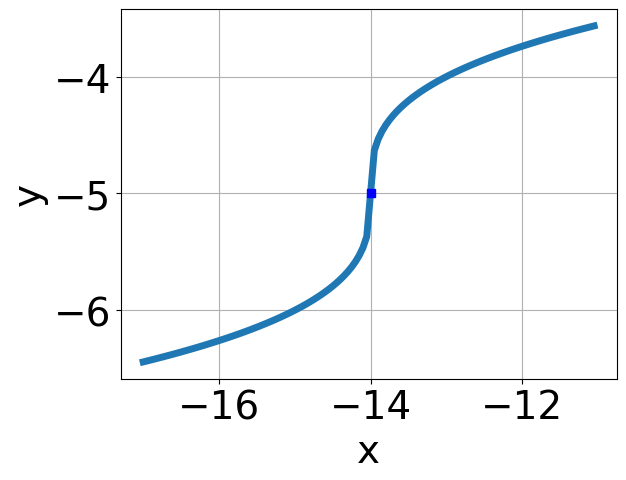
\includegraphics[width = 0.3\textwidth]{../Figures/radicalEquationToGraphAA.png}\item 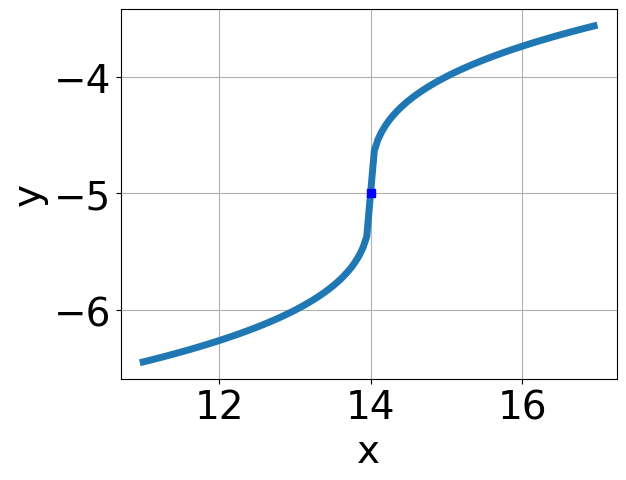
\includegraphics[width = 0.3\textwidth]{../Figures/radicalEquationToGraphBA.png}\item 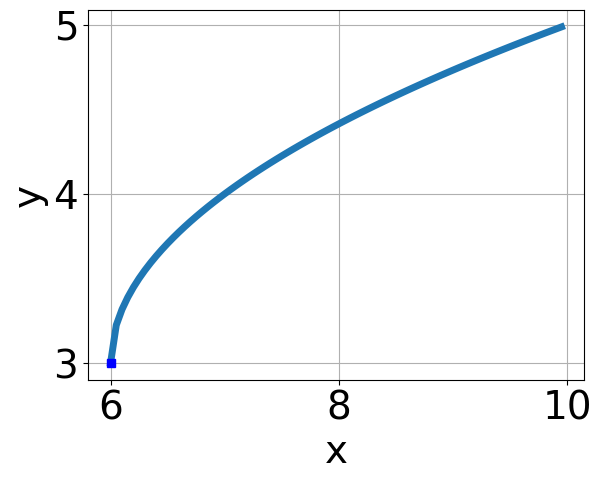
\includegraphics[width = 0.3\textwidth]{../Figures/radicalEquationToGraphCA.png}\item 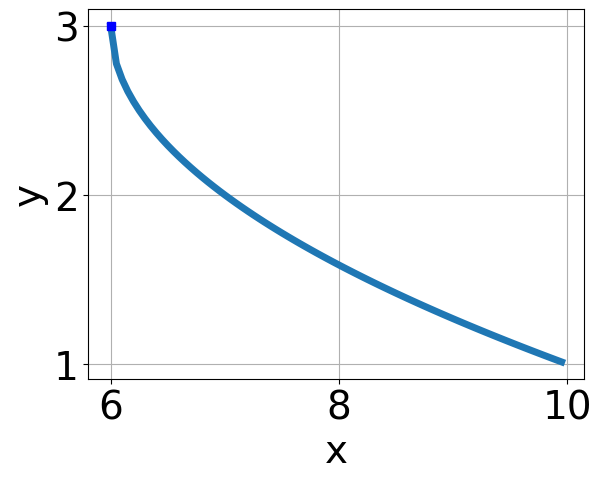
\includegraphics[width = 0.3\textwidth]{../Figures/radicalEquationToGraphDA.png}\end{multicols}\item None of the above.
\end{enumerate} }
\litem{
Solve the radical equation below. Then, choose the interval(s) that the solution(s) belongs to.\[ \sqrt{-4 x - 7} - \sqrt{-2 x - 2} = 0 \]\begin{enumerate}[label=\Alph*.]
\item \( x_1 \in [-3.14, -1.9] \text{ and } x_2 \in [-2.62,-1.4] \)
\item \( x \in [-3.14,-1.9] \)
\item \( \text{All solutions lead to invalid or complex values in the equation.} \)
\item \( x_1 \in [-2.06, -0.67] \text{ and } x_2 \in [-1.41,-0.79] \)
\item \( x \in [-5.15,-3.82] \)

\end{enumerate} }
\litem{
Choose the graph of the equation below.\[ f(x) = \sqrt{x - 12} + 6 \]\begin{enumerate}[label=\Alph*.]
\begin{multicols}{2}\item 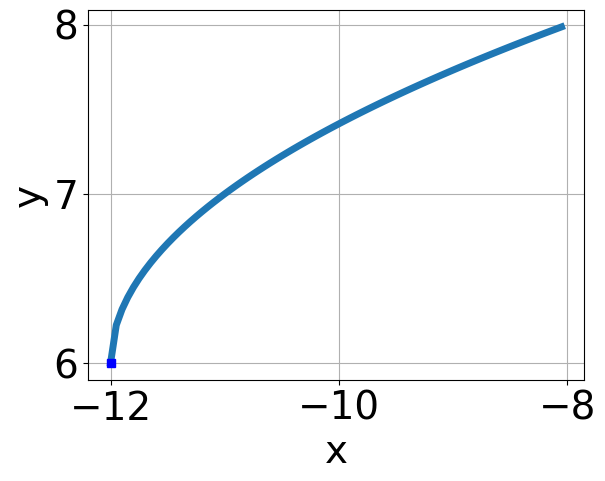
\includegraphics[width = 0.3\textwidth]{../Figures/radicalEquationToGraphCopyAA.png}\item 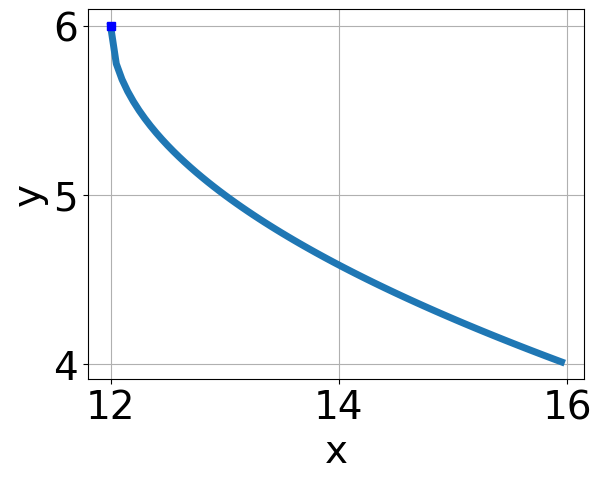
\includegraphics[width = 0.3\textwidth]{../Figures/radicalEquationToGraphCopyBA.png}\item 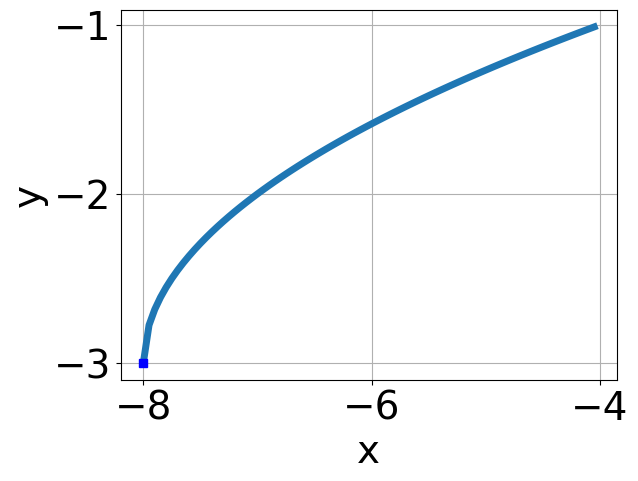
\includegraphics[width = 0.3\textwidth]{../Figures/radicalEquationToGraphCopyCA.png}\item 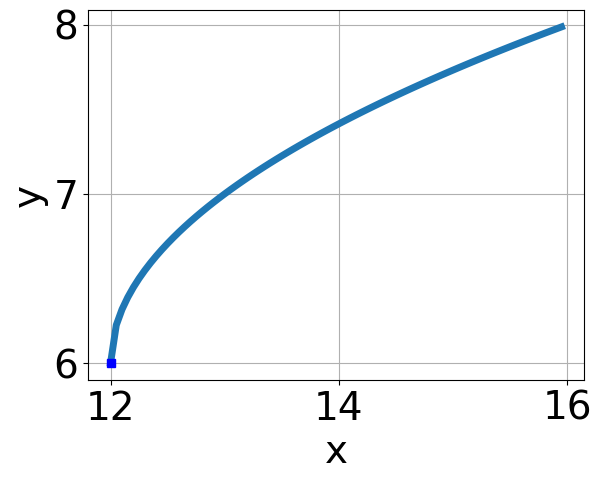
\includegraphics[width = 0.3\textwidth]{../Figures/radicalEquationToGraphCopyDA.png}\end{multicols}\item None of the above.
\end{enumerate} }
\litem{
Solve the radical equation below. Then, choose the interval(s) that the solution(s) belongs to.\[ \sqrt{3 x + 5} - \sqrt{4 x - 2} = 0 \]\begin{enumerate}[label=\Alph*.]
\item \( x_1 \in [-3.1, 0.6] \text{ and } x_2 \in [6,10] \)
\item \( x \in [2.9,4.4] \)
\item \( \text{All solutions lead to invalid or complex values in the equation.} \)
\item \( x \in [6.2,7.2] \)
\item \( x_1 \in [-3.1, 0.6] \text{ and } x_2 \in [-3.5,3.5] \)

\end{enumerate} }
\end{enumerate}

\end{document}